\chapter{Results and Analysis}
\label{chapter:results-analysis}
	
	In this chapter, we begin an analysis of 1D heterogeneous systems first, then move our attention to 2D heterogeneous systems. Although 1D homogeneous systems were simulated, they did not provide any interesting or new insight into diffusive behaviour, therefore those simulations and analytical data are not presented in detail. We begin each section with selected images of simulated density distributions to motivate further analysis. More specifically, we analyze how changing the boundary transition probabilities, region diffusivities, and cell geometry (2D only), affects the mean-squared-displacement (MSD) and show that sub- and super-diffusive regimes exist. Lastly, we show that the long-time effective diffusivity is non-trivial even for simple-cell geometries.
	 
\section{1D Systems}
\label{sec:ra-1D}
	For very large systems or short simulation times---conditions where the density distribution is zero at the absolute boundaries---agreement between the Monte Carlo (MC) and master equation (ME) simulation solutions, and analytical solutions (\ref{eq:1D-diffusion-equation-solution}) of the 1D diffusion equation with no net drift and constant diffusion factor (\ref{eq:1D-diffusion-equation}), was observed (Figure \ref{fig:11U_homogeneous_plots_1D}). 

	\begin{figure}[h]
		\centering
		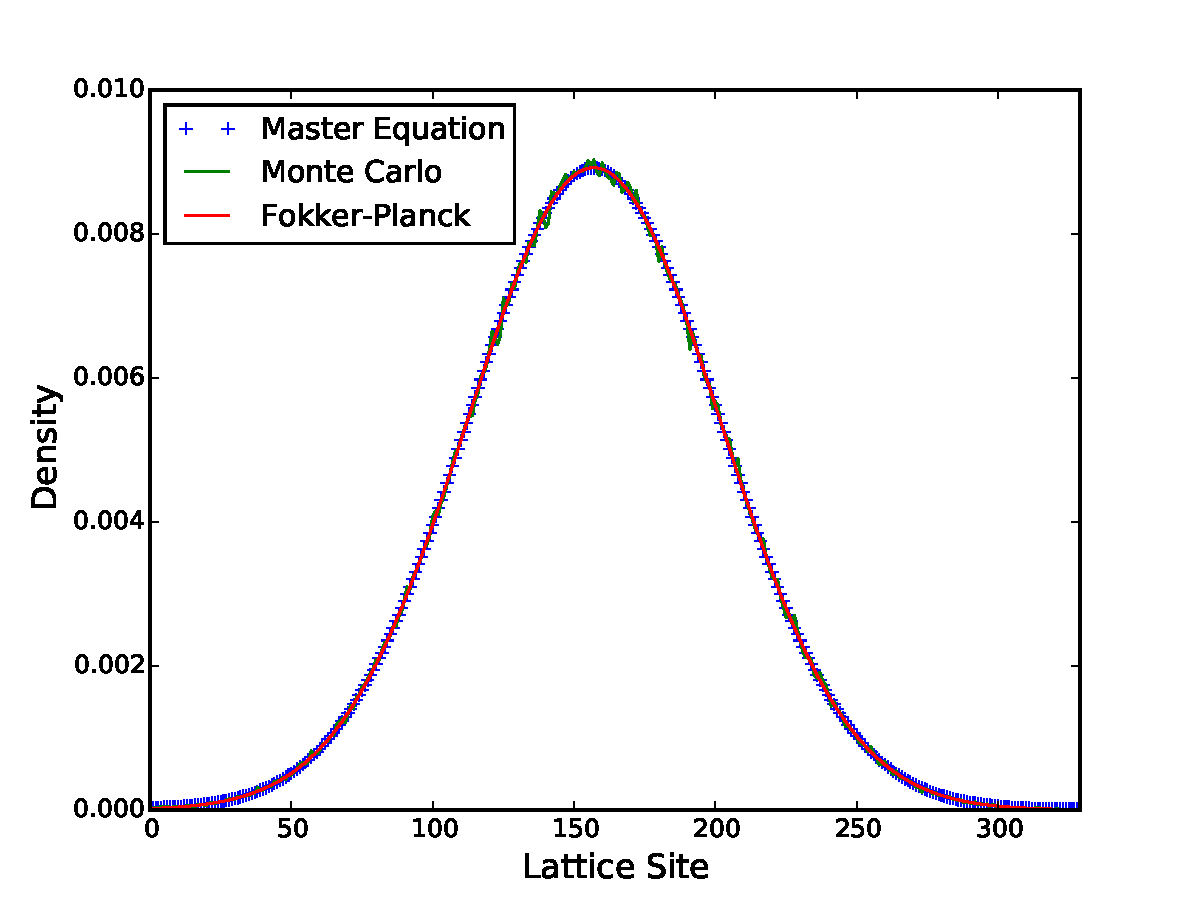
\includegraphics[width=1.0\linewidth]{../images/1D/11U_homogeneous_plots_1D}
		\caption{Simple 1D system with no internal semi-permeable boundaries. Simulation solutions plotted for ME and MC methods. Additionally, an exact solution to diffusion equation (Fokker-Planck) is plotted. Parameter specifications: 330 lattice sites, $ D = 0.1 $, $ N = 8\cdot10^5 $ particles in MC simulation, and density normalized.}
		\label{fig:11U_homogeneous_plots_1D}
	\end{figure}
	
	The 1D diffusion equation \ref{eq:1D-diffusion-equation} may be known as a `simple' Fokker-Planck or Smoluchowski equation and is sometimes utilized as a model of classical Brownian motion.
	
	\begin{equation}
	\label{eq:1D-diffusion-equation}
		\frac{\partial\rho(x,t)}{\partial t} = D_0 \frac{\partial^2 \rho(x,t)}{\partial x^2}
	\end{equation}
	
	Assuming that $ N $ particles start from the origin, Equation \ref{eq:1D-diffusion-equation} has the solution:
	
	\begin{equation}
	\label{eq:1D-diffusion-equation-solution}
		\rho(x,t)=\frac{N}{\sqrt{4\pi Dt}}e^{-\frac{x^2}{4Dt}}
	\end{equation}	
	
	Equation \ref{eq:1D-diffusion-equation-solution} was used to create the Fokker-Planck plot in Figure \ref{fig:11U_homogeneous_plots_1D}. The solution to \ref{eq:1D-diffusion-equation} is not a solution to a boundary value problem. For example, it is possible to solve \ref{eq:1D-diffusion-equation} for reflecting absolute boundary conditions: $ \rho_x(0,t) = \rho_x(L,t) = 0 $. It is even possible to solve it for `repeating' boundary conditions that represent semi-permeable internal boundaries (Jessica Cervi's thesis); these specific problems were not explored and are not discussed further. However, it is comparatively easy to obtain a solution to such a system with internal semi-permeable and absolute reflecting boundaries by utilizing MC and ME methods for the simulation of the system; Figure \ref{fig:11U_heterogeneous_plots_1D} shows such a solution.
	
	With reference to Figure \ref{fig:11U_homogeneous_plots_1D}, note the good agreement between the ME and MC simulation solutions and analytical solution. The ME simulation solution and analytical solution are perfectly superimposed. The MC simulation shows characteristic statistical fluctuations that reflect the underlying `random' movement of individual particles in the simulation. The relative magnitude of these fluctuations decreases with an increasing number of particles $ N $ according to $ 1/\sqrt{N} $.

	\begin{figure}[h]
		\centering
		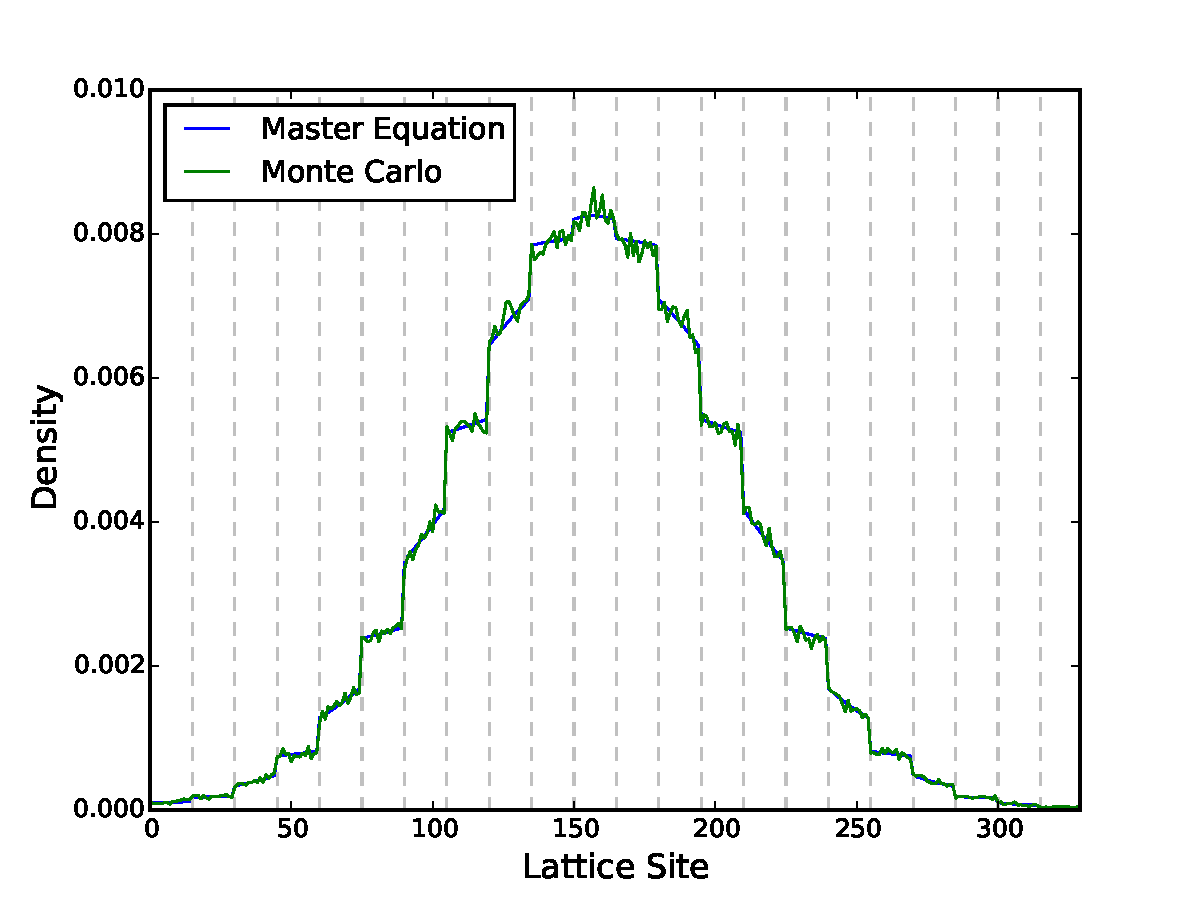
\includegraphics[width=1.0\linewidth]{../images/1D/11U_heterogeneous_plots_1D}
		\caption{1D heterogeneous system with internal semi-permeable boundaries. Simulation solutions plotted for ME and MC methods. Parameter specifications: 330 lattice sites, 15 lattice sites per cellular or extracellular region, $ D_i = 0.05 $, $ D_e = 0.2 $, and $ P_{i\rightarrow e} = 0.05 $. $ N = 5 \cdot 10^5 $ particles in the MC simulation and density normalized. Vertical dashed lines show semi-permeable boundary positions.}
		\label{fig:11U_heterogeneous_plots_1D}
	\end{figure}
	
	Statistical fluctuations in the MC simulation solution are more visible in Figure \ref{fig:11U_heterogeneous_plots_1D}. The ME simulation was orders of magnitude faster in reaching completion and does not show any fluctuations since the density distribution is evolved in time under the assumption that there are \textsl{very} many particles at each lattice site. It is expected that in the limit of an infinite number of particles, the MC solution converges to the ME solution. Comparisons to analytical or numerical solutions of the Fokker-Planck equation were not made but doing so may be of interest in the future.
	
	\begin{figure}[h]
		\centering
		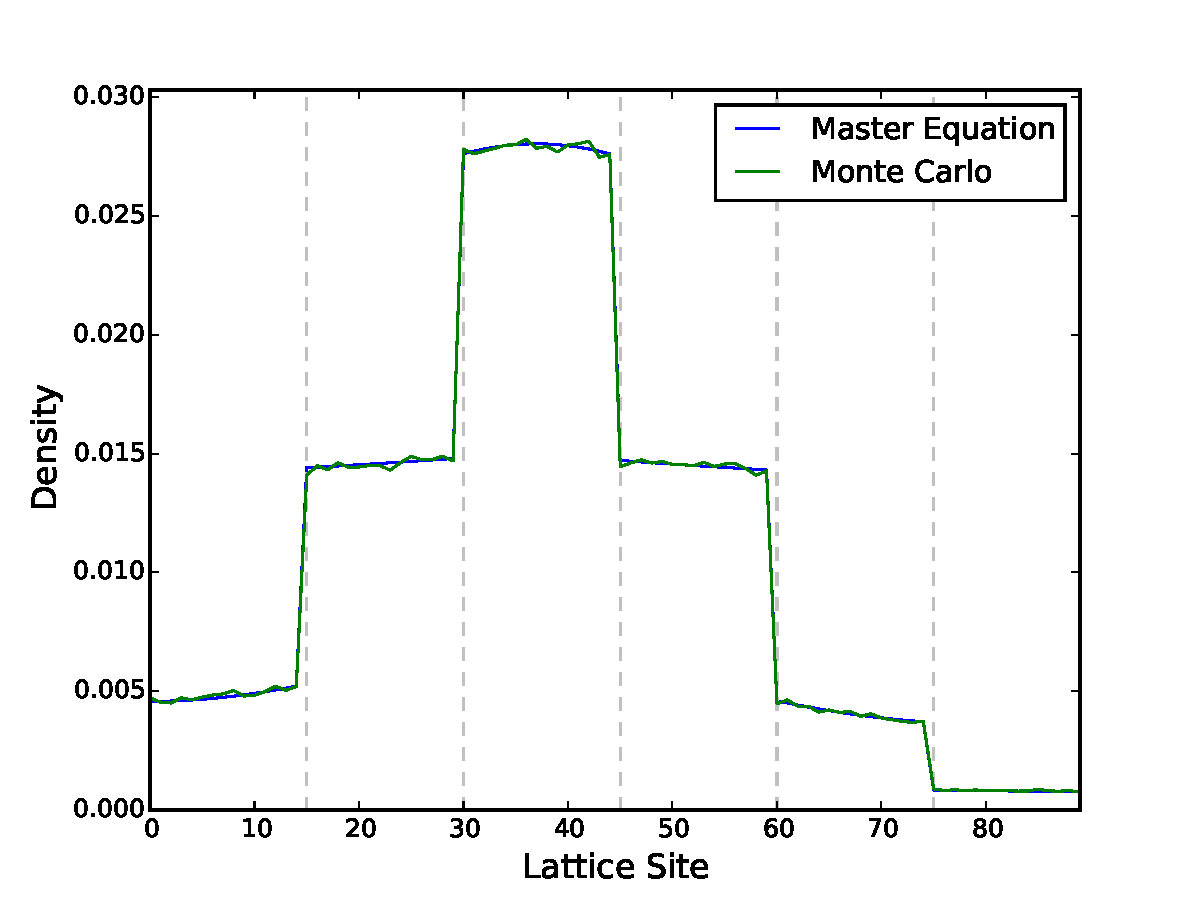
\includegraphics[width=1.0\linewidth]{../images/1D/3U_heterogeneous_plots_1D}
		\caption{1D heterogeneous system with internal semi-permeable boundaries. Simulation solutions plotted for ME and MC methods. Parameter specifications: 90 lattice sites, 15 lattice sites per cellular or extracellular region, $ D_i = 0.05 $, $ D_e = 0.2 $, and $ P_{i\rightarrow e} = 0.01 $. $ N = 8 \cdot 10^5 $ particles in the MC simulation and density normalized. Vertical dashed lines show semi-permeable boundary positions.}
		\label{fig:3U_heterogeneous_plots_1D}
	\end{figure}
	
	Interesting to note in Figure \ref{fig:11U_heterogeneous_plots_1D} and \ref{fig:3U_heterogeneous_plots_1D}, the magnitude of the fluctuations in the MC solution appear larger at higher densities and smaller at lower densities. In Figure \ref{fig:11U_heterogeneous_plots_1D}, extracellular regions with 4-times larger diffusivity equilibrate faster than the cellular regions; this is visible as `flat' versus `sloped' density distributions. Figure \ref{fig:3U_heterogeneous_plots_1D} shows behaviour at the absolute reflecting boundaries.
	
	\begin{figure}[h]
		\centering
		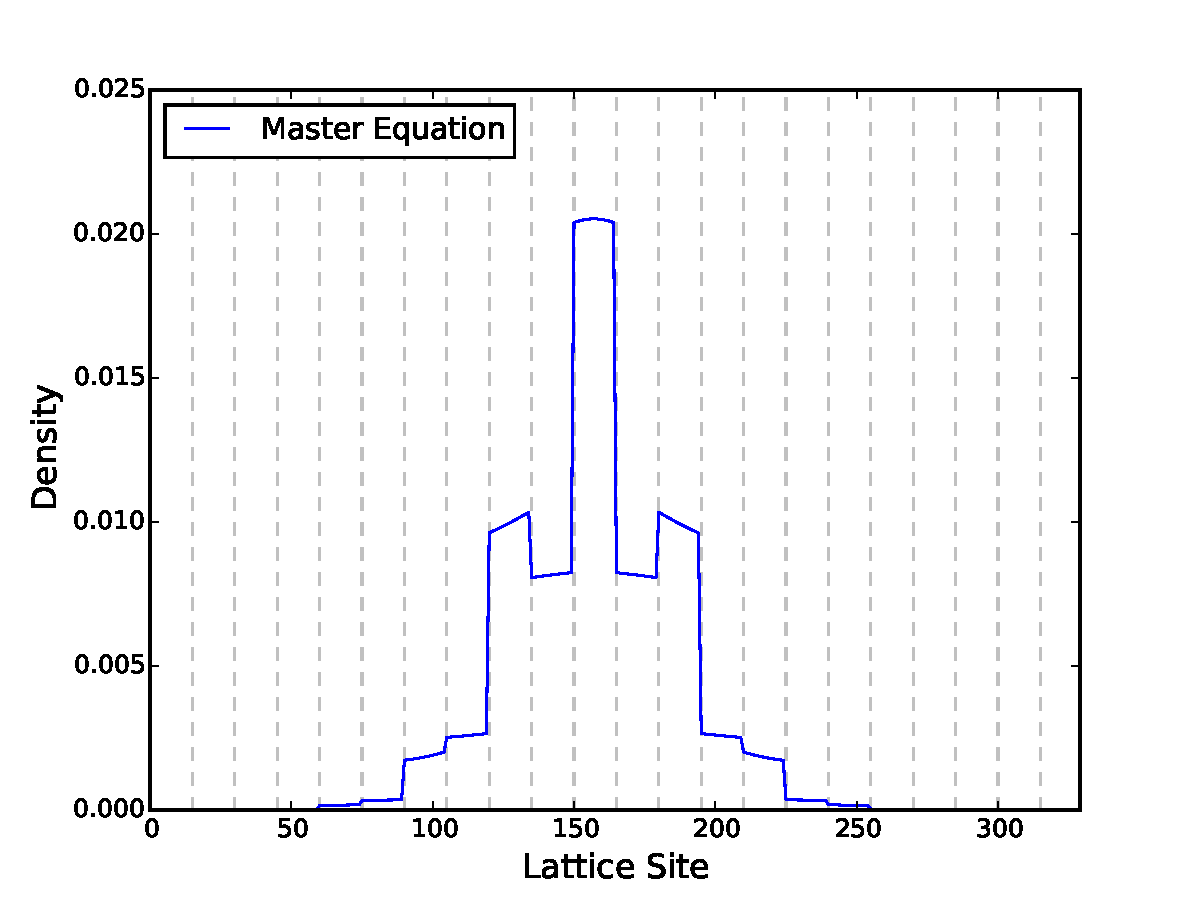
\includegraphics[width=1.0\linewidth]{../images/1D/11U_heterogeneous_plots_1D_nonphysical}
		\caption{1D heterogeneous system with internal semi-permeable boundaries. Non-physical density distribution simulated by violating the semi-permeable boundary condition (sometimes known as the isothermal boundary condition). Parameter specifications: 330 lattice sites, 15 lattice sites per cellular or extracellular region, $ D_i = 0.05 $, $ D_e = 0.2 $, and $ P_{i\rightarrow e} = 0.01 $ and $ P_{e\rightarrow i} =  0.005 $. Correctly chosen, $ P_{e\rightarrow i} =  0.0025 $. Vertical dashed lines show semi-permeable boundary positions. }
		\label{fig:11U_heterogeneous_plots_1D_nonphysical}
	\end{figure}
	
	Figure \ref{fig:11U_heterogeneous_plots_1D_nonphysical} shows the necessity of having coupled transition probabilities for the semi-permeable boundaries. The distribution in the long-time limit does not approach a uniform distribution, as would be expected for any system with passive semi-permeable boundaries and reflecting absolute boundaries. In the long-time, the density grows in certain cells and shrinks in others, similar to what might be expected if the semi-permeable boundaries behaved in an active-selective manner. 

\subsection{Total Transition Probability}
	
	\begin{figure}[h]
		\centering
		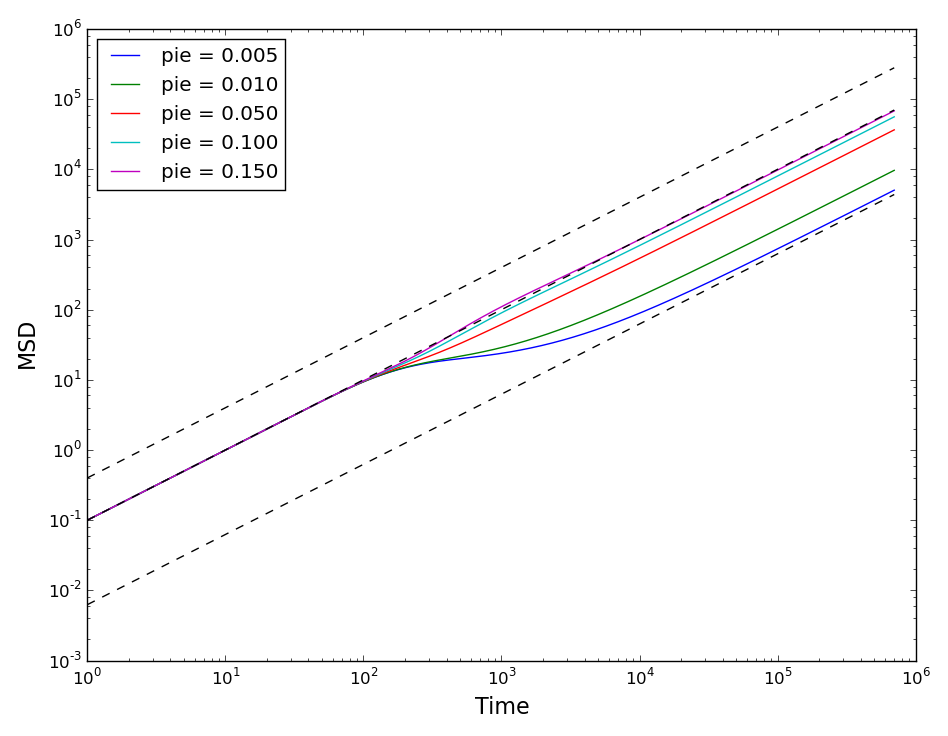
\includegraphics[width=1.0\linewidth]{../images/1D/pie_msd_1D}
		\caption{}
		\label{fig:pie_msd_1D}
	\end{figure}
	
	\begin{figure}[h]
		\centering
		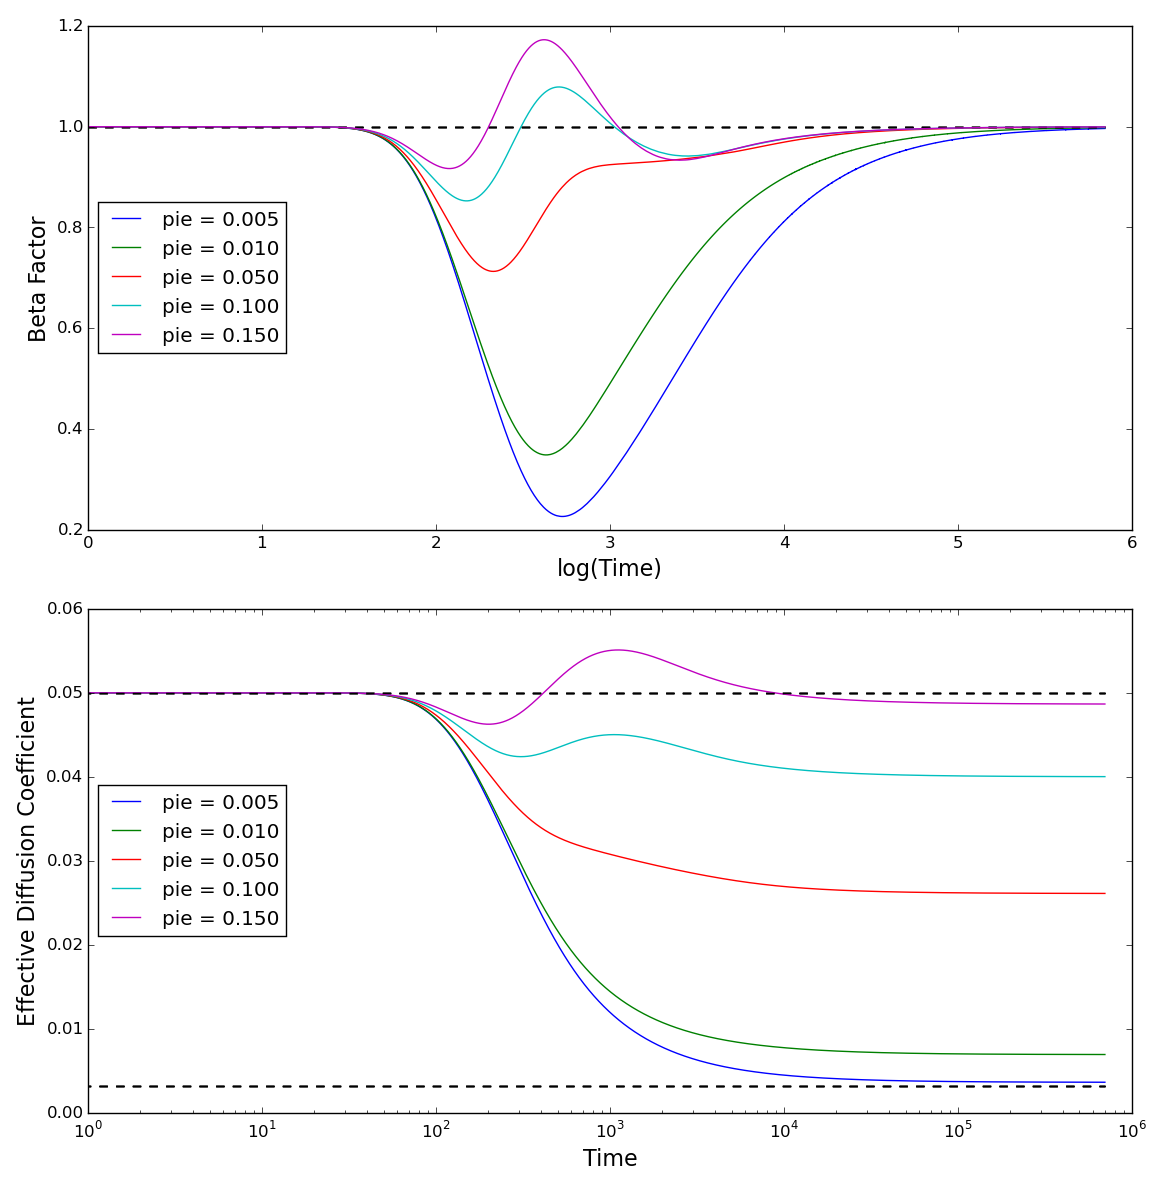
\includegraphics[width=1.0\linewidth]{../images/1D/pie_beta_deff_1D}
		\caption{}
		\label{fig:pie_beta_deff_1D}
	\end{figure}

\subsection{Cellular and Extracellular Diffusivities}
	
	\begin{figure}[h]
		\centering
		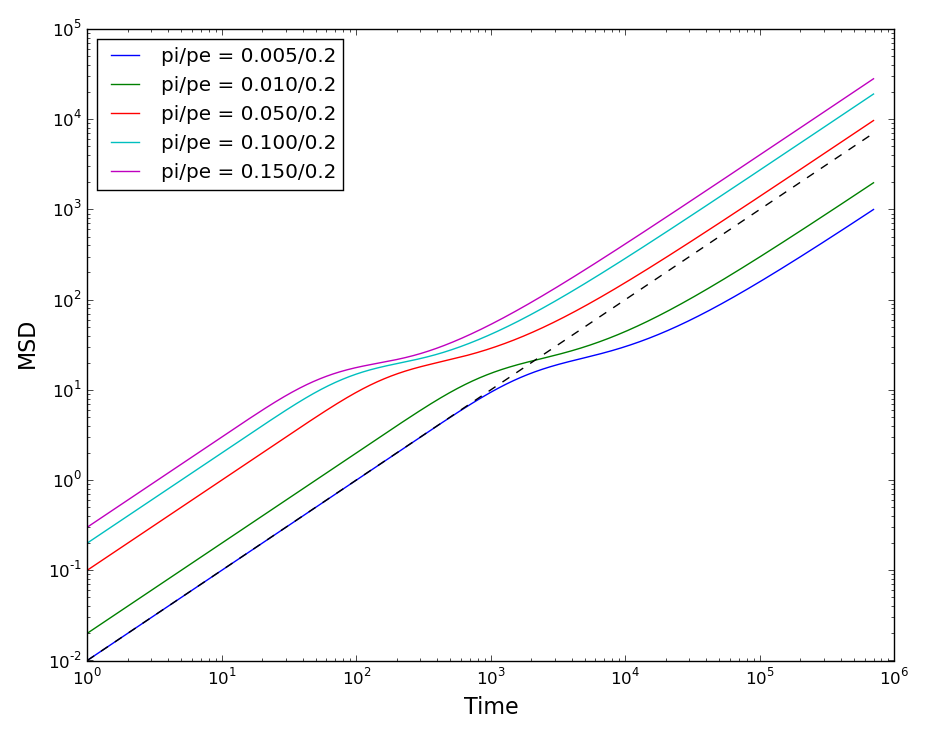
\includegraphics[width=1.0\linewidth]{../images/1D/pipe_msd_1D}
		\caption{}
		\label{fig:pipe_msd_1D}
	\end{figure}
	
	\begin{figure}[h]
		\centering
		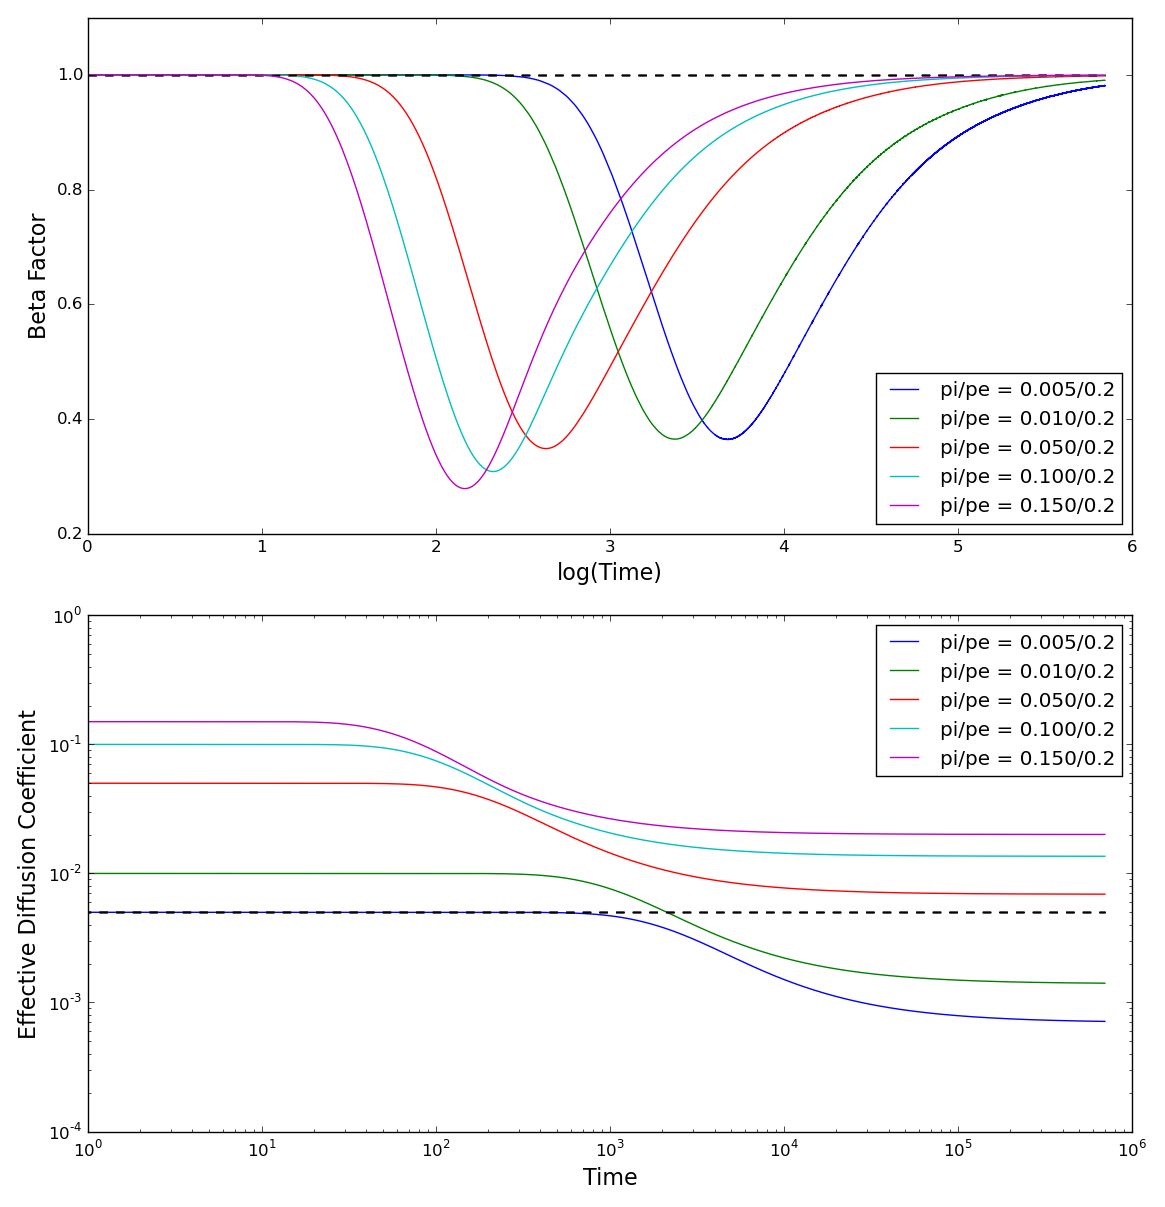
\includegraphics[width=1.0\linewidth]{../images/1D/pipe_beta_deff_1D}
		\caption{}
		\label{fig:pipe_beta_deff_1D}
	\end{figure}

\newpage
\section{2D Systems}
\label{sec:ra-2D}

	Hello begin by writing.
	\begin{figure}[h]
		\centering
		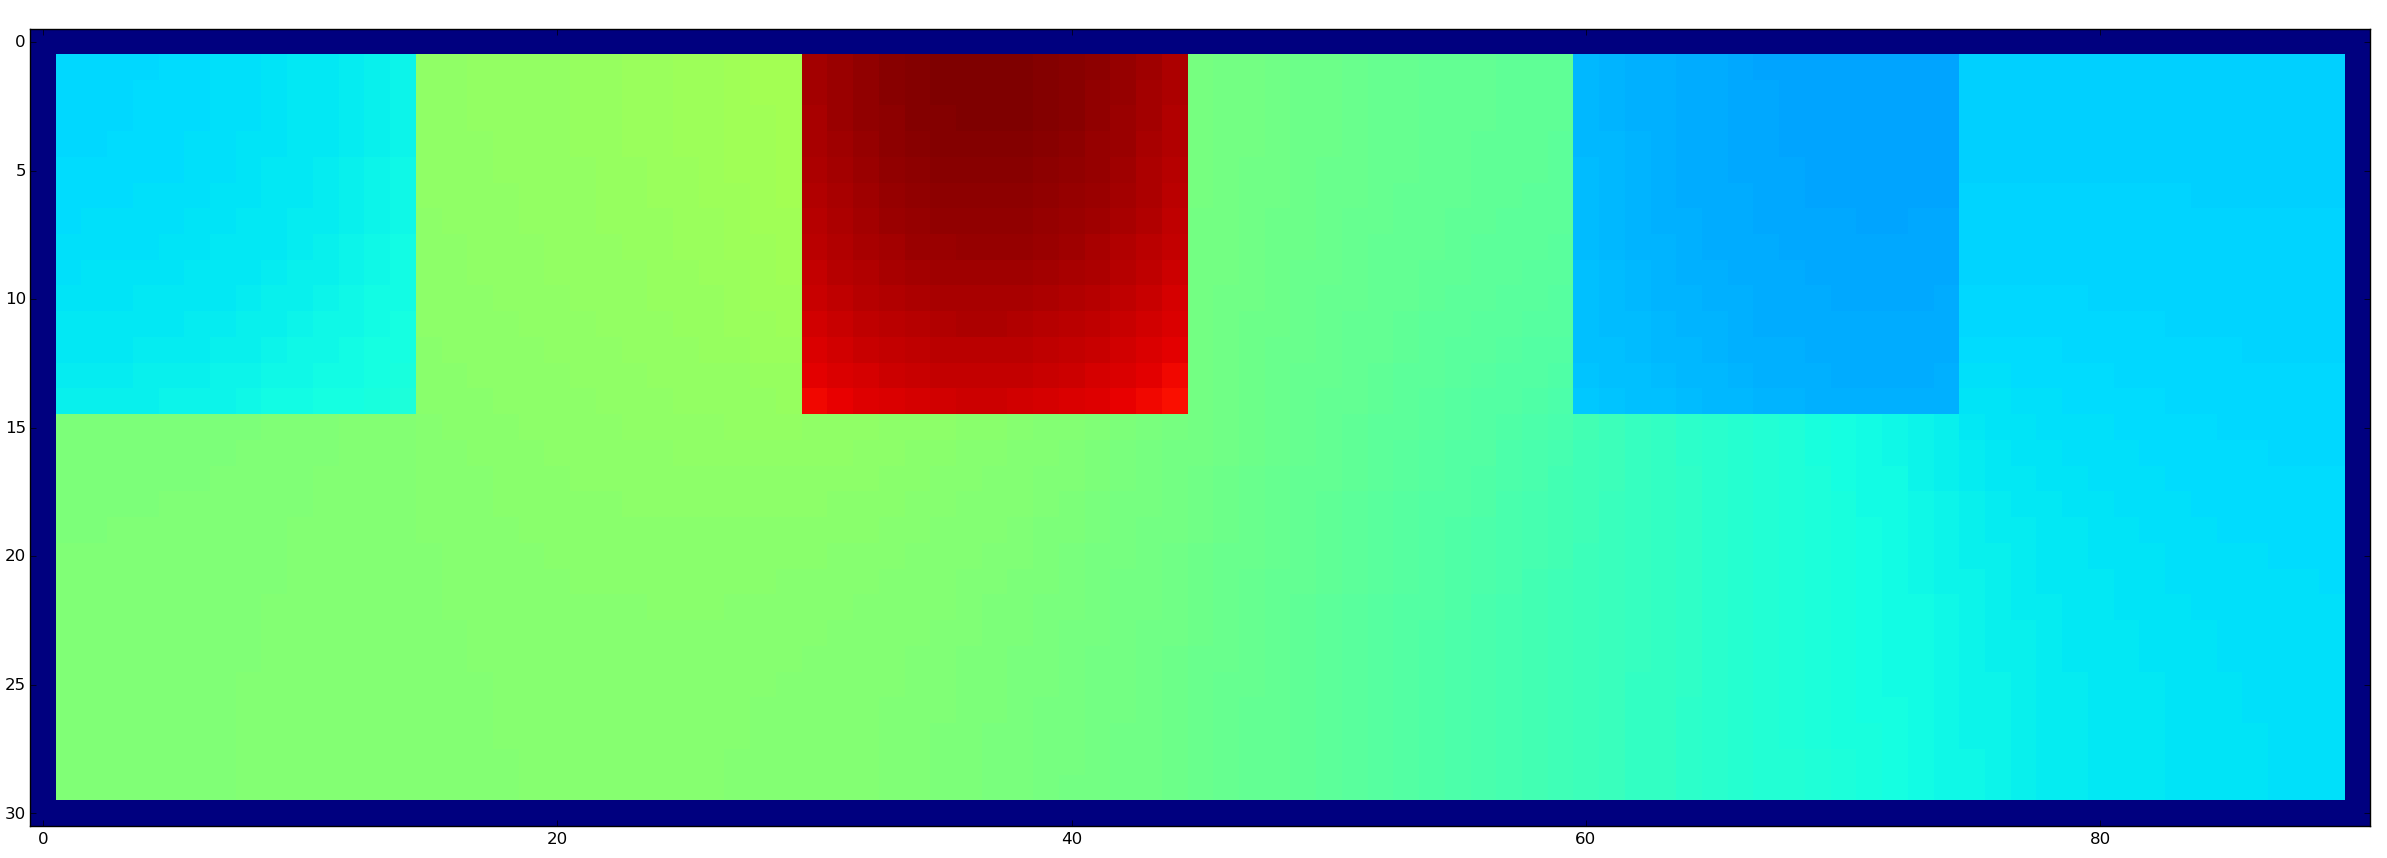
\includegraphics[width=1.0\linewidth]{../images/2D/heterogeneous_3U_2D}
		\caption{}
		\label{fig:heterogeneous_3U_2D}
	\end{figure}
	
	\begin{figure}[h]
		\centering
		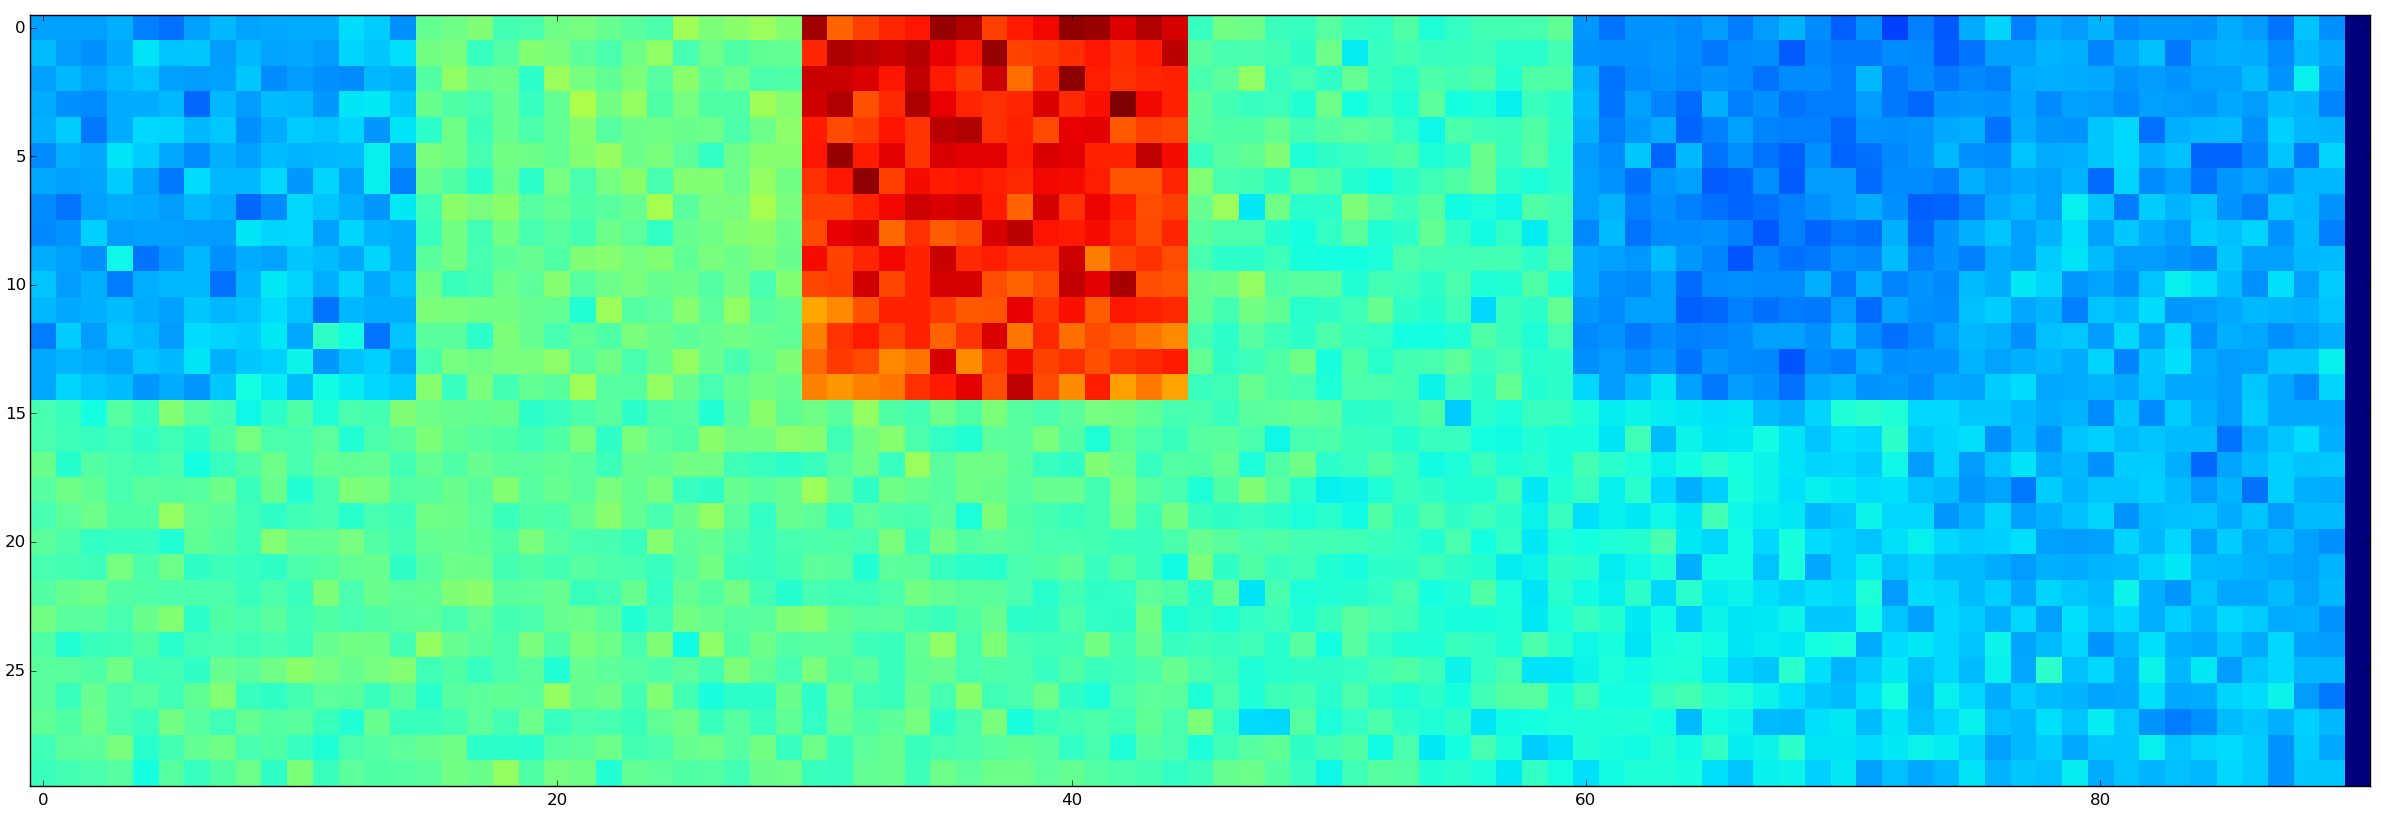
\includegraphics[width=1.0\linewidth]{../images/2D/MC_heterogeneous_3U_2D}
		\caption{}
		\label{fig:MC_heterogeneous_3U_2D}
	\end{figure}
	
	\begin{figure}[h]
		\centering
		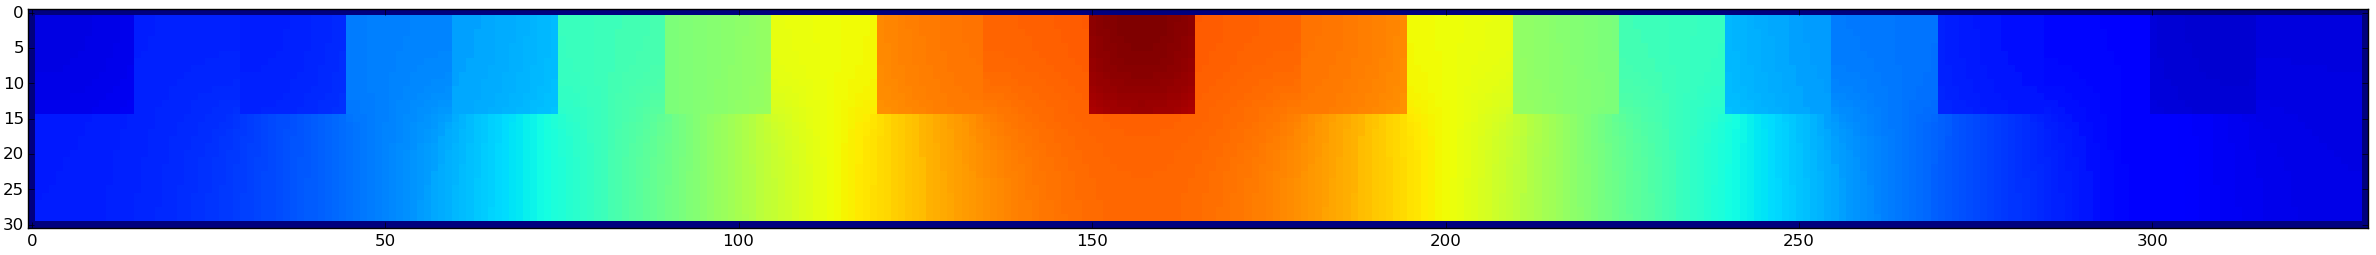
\includegraphics[width=1.0\linewidth]{../images/2D/heterogeneous_11U_2D}
		\caption{}
		\label{fig:heterogeneous_11U_2D}
	\end{figure}
	
	\begin{figure}[h]
		\centering
		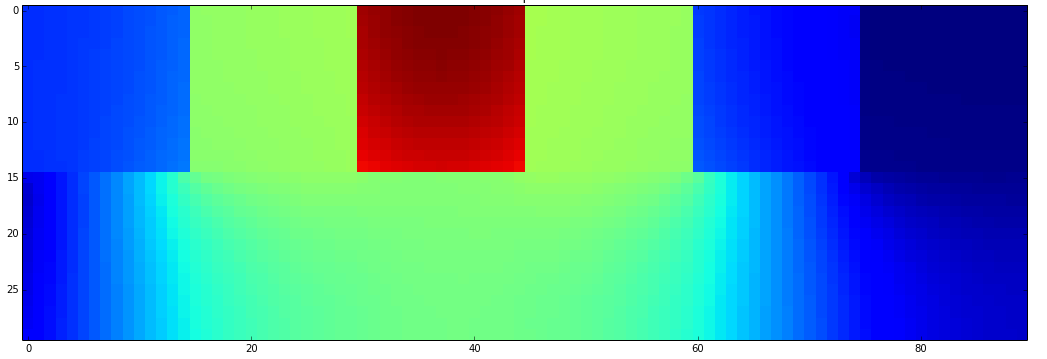
\includegraphics[width=1.0\linewidth]{../images/2D/error_in_diffusion}
		\caption{}
		\label{fig:error_in_diffusion}
	\end{figure}
	
	\begin{figure}[h]
		\centering
		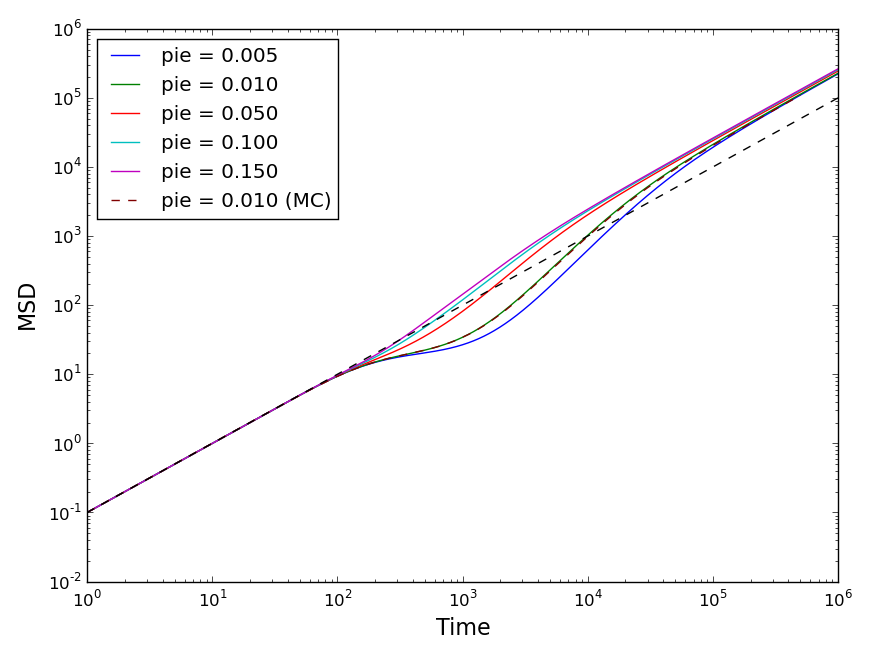
\includegraphics[width=1.0\linewidth]{../images/2D/pie_msd_2D}
		\caption{}
		\label{fig:pie_msd_2D}
	\end{figure}
	
	\begin{figure}[h]
		\centering
		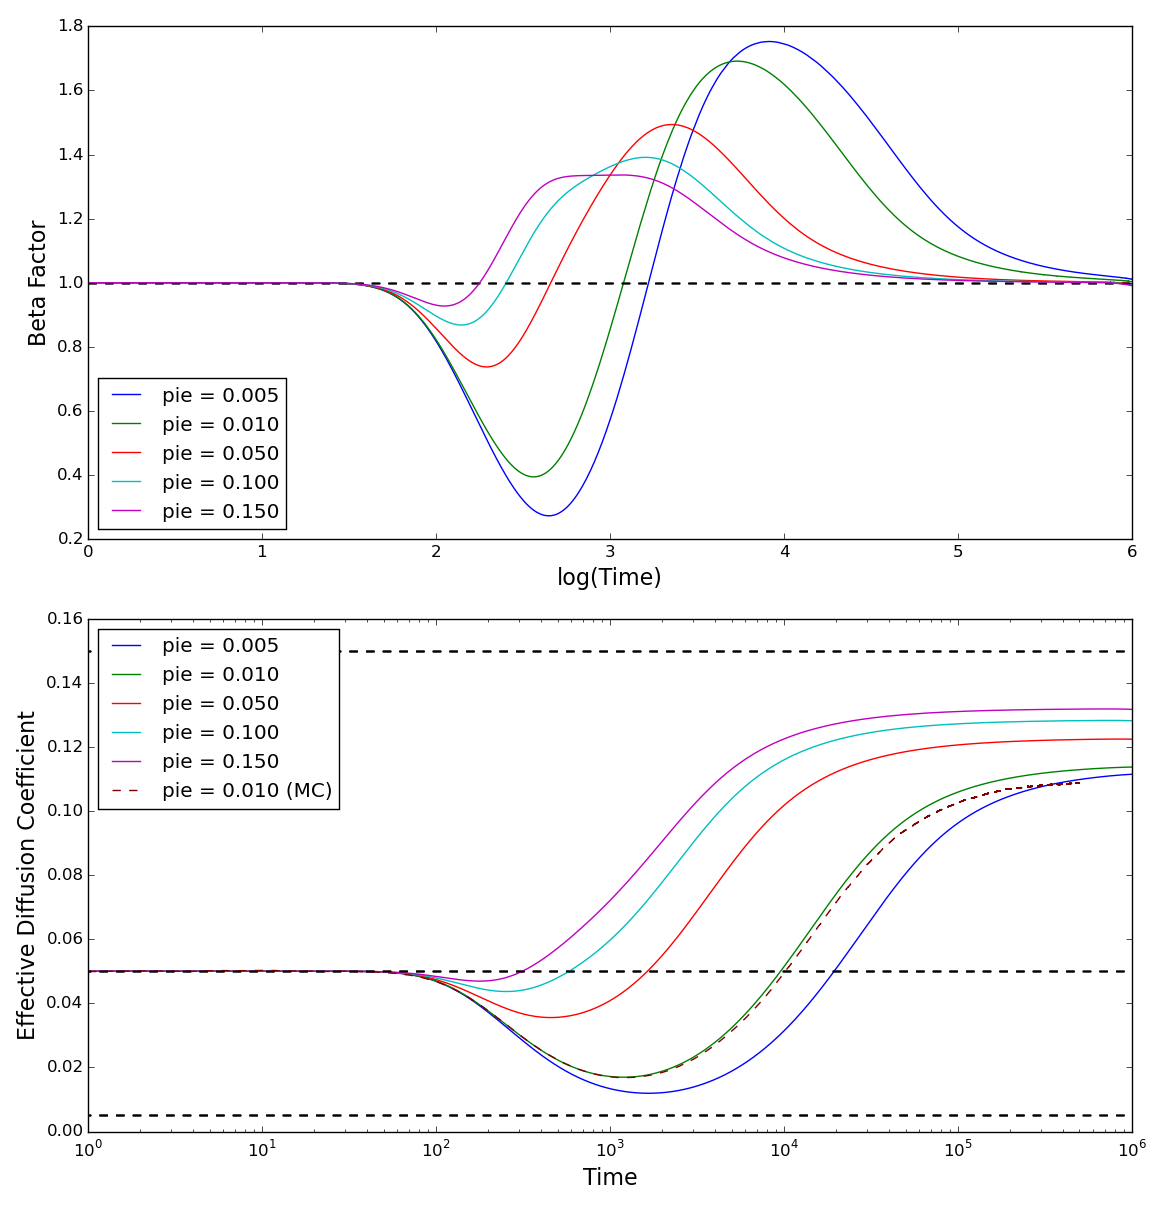
\includegraphics[width=1.0\linewidth]{../images/2D/pie_beta_deff_2D}
		\caption{}
		\label{fig:pie_beta_deff_2D}
	\end{figure}
	
	\begin{figure}[h]
		\centering
		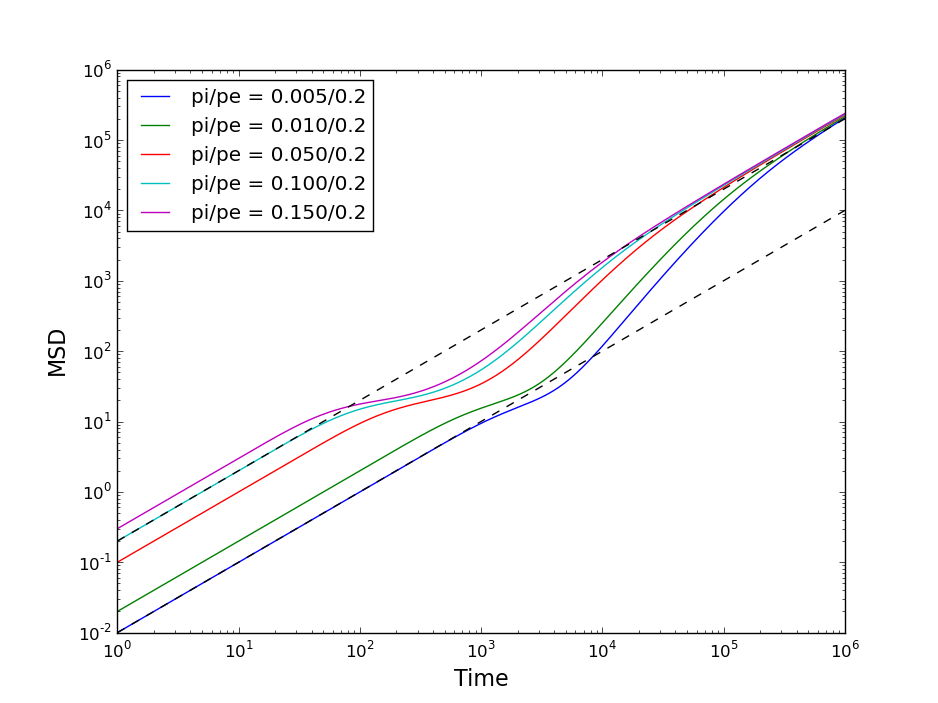
\includegraphics[width=1.0\linewidth]{../images/2D/pipe_msd_2D}
		\caption{}
		\label{fig:pipe_msd_2D}
	\end{figure}
	
	\begin{figure}[h]
		\centering
		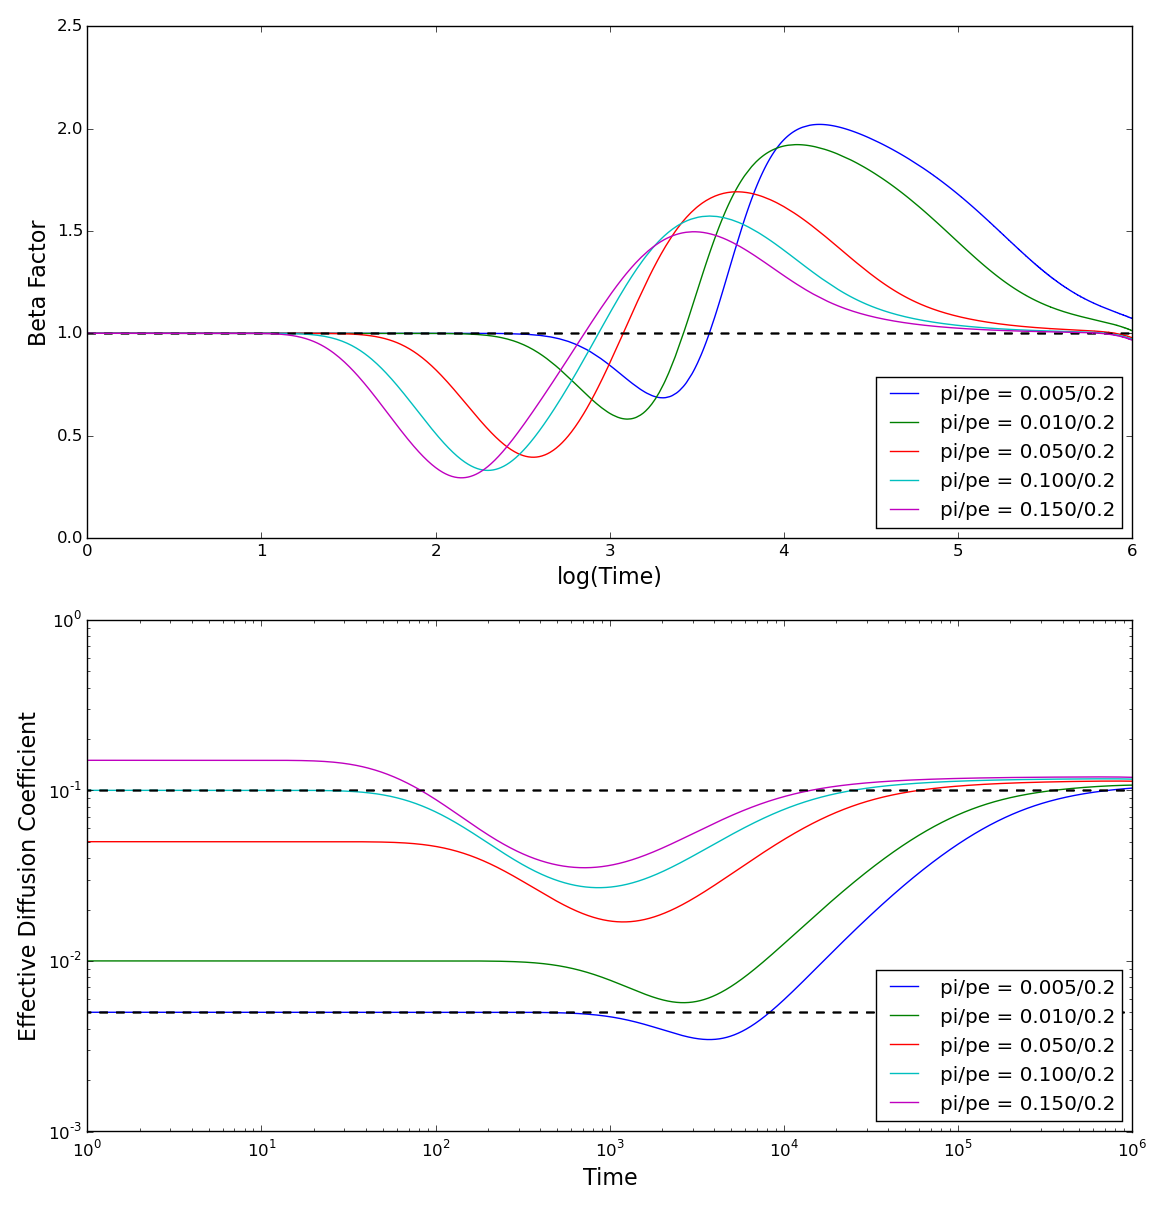
\includegraphics[width=1.0\linewidth]{../images/2D/pipe_beta_deff_2D}
		\caption{}
		\label{fig:pipe_beta_deff_2D}
	\end{figure}
	
	\begin{figure}[h]
		\centering
		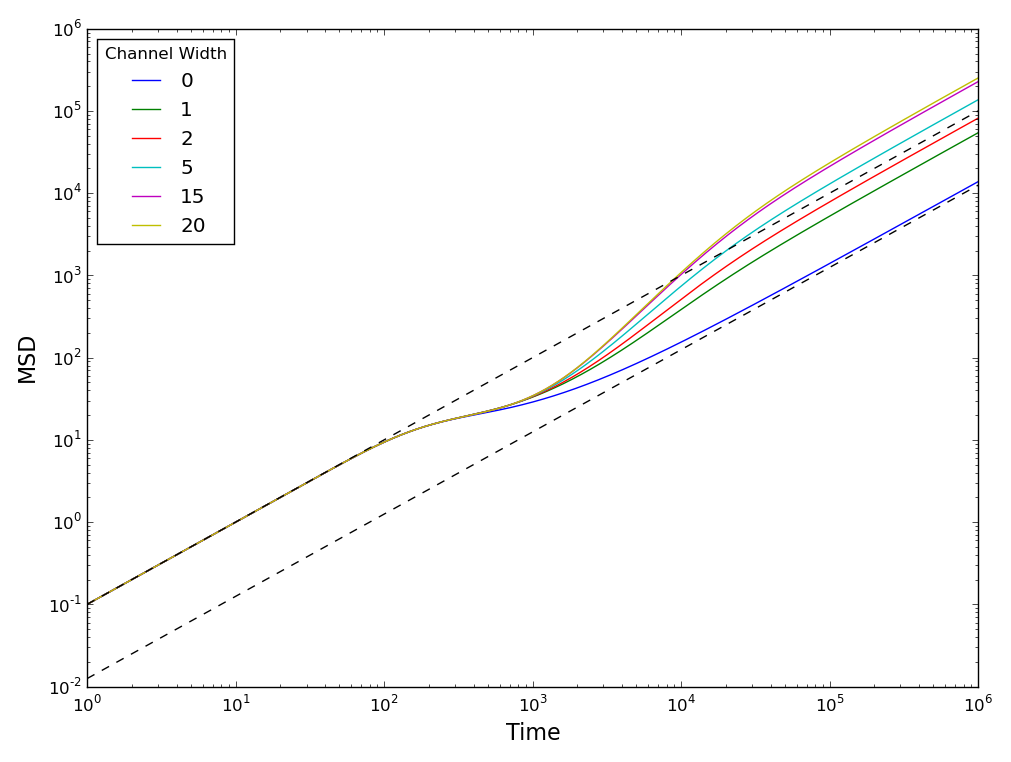
\includegraphics[width=1.0\linewidth]{../images/2D/ye_msd_2D}
		\caption{}
		\label{fig:ye_msd_2D}
	\end{figure}
	
	\begin{figure}[h]
		\centering
		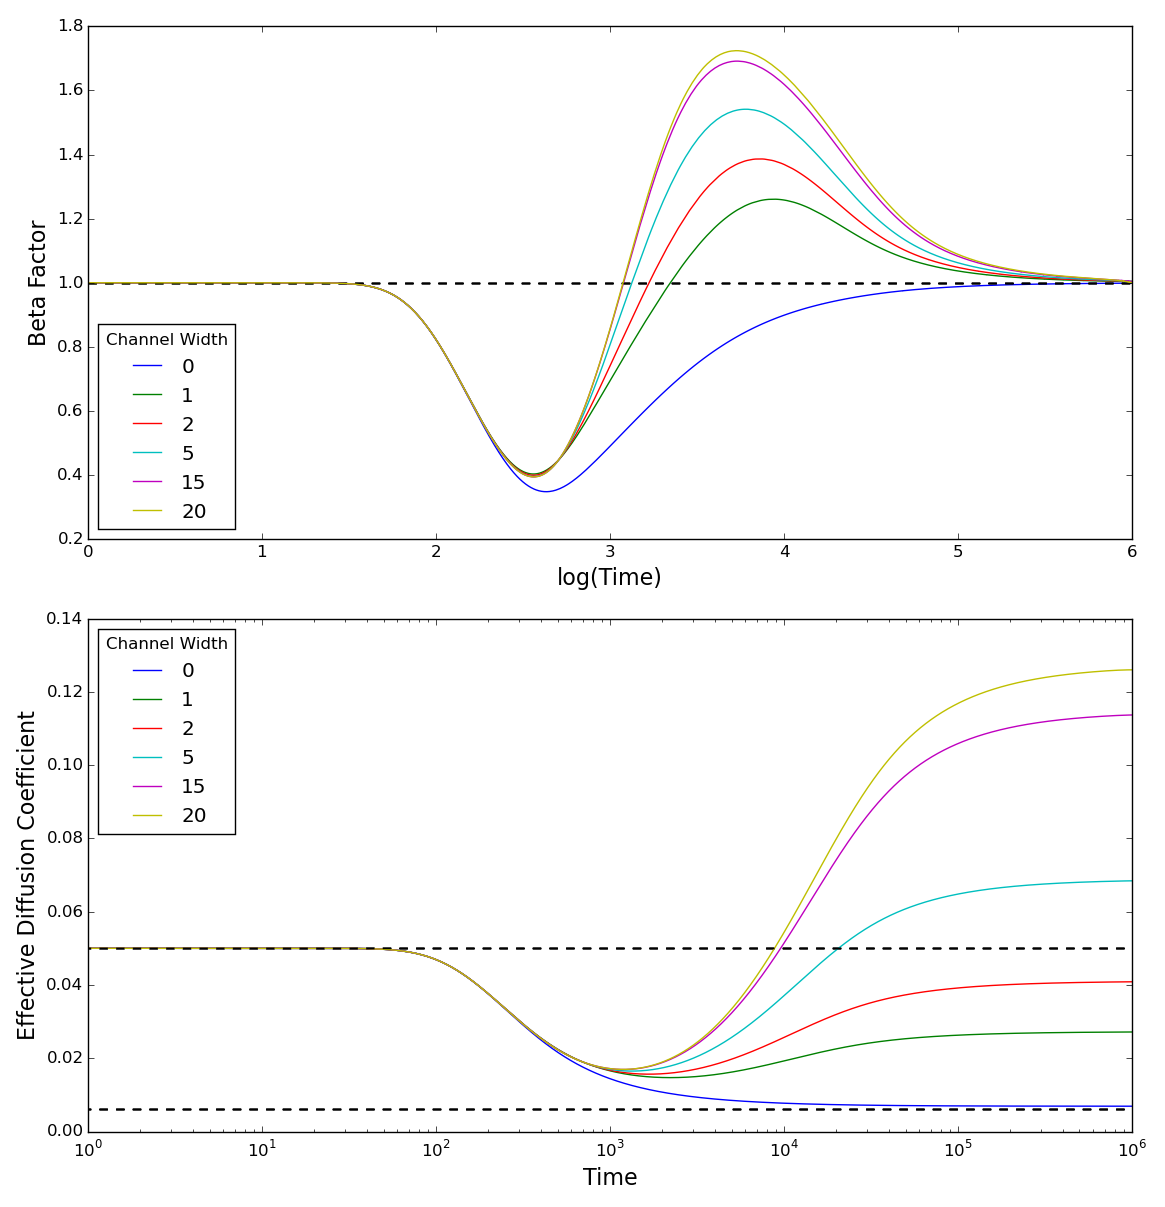
\includegraphics[width=1.0\linewidth]{../images/2D/ye_beta_deff_2D}
		\caption{}
		\label{fig:ye_beta_deff_2D}
	\end{figure}

	